\documentclass[compress]{beamer}
\usepackage{ifthen,verbatim}

\newcommand{\isnote}{}
\xdefinecolor{lightyellow}{rgb}{1.,1.,0.25}
\xdefinecolor{darkblue}{rgb}{0.1,0.1,0.7}
\xdefinecolor{darkred}{rgb}{0.9,0.,0.}
\xdefinecolor{lightblue}{rgb}{0.2,0.6,0.6}

%% Uncomment this to get annotations
%% \def\notes{\addtocounter{page}{-1}
%%            \renewcommand{\isnote}{*}
%% 	   \beamertemplateshadingbackground{lightyellow}{white}
%%            \begin{frame}
%%            \frametitle{Notes for the previous page (page \insertpagenumber)}
%%            \itemize}
%% \def\endnotes{\enditemize
%% 	      \end{frame}
%%               \beamertemplateshadingbackground{white}{white}
%%               \renewcommand{\isnote}{}}

%% Uncomment this to not get annotations
\def\notes{\comment}
\def\endnotes{\endcomment}

\setbeamertemplate{navigation symbols}{}
\setbeamertemplate{headline}{\mbox{ } \hfill
\begin{minipage}{5.5 cm}
\vspace{-0.75 cm} \small
\end{minipage} \hfill
\begin{minipage}{4.5 cm}
\vspace{-0.75 cm} \small
\begin{flushright}
\ifthenelse{\equal{\insertpagenumber}{1}}{}{Jim Pivarski \hspace{0.2 cm} \insertpagenumber\isnote/\pageref{numpages}}
\end{flushright}
\end{minipage}\mbox{\hspace{0.2 cm}}\includegraphics[height=1 cm]{../cmslogo} \hspace{0.1 cm} \includegraphics[height=1 cm]{../tamulogo} \hspace{0.01 cm} \vspace{-1.05 cm}}

\begin{document}
\begin{frame}
\vfill
\begin{center}
\textcolor{darkblue}{\Large Magnetic field information from muon alignment}

\vfill
\begin{columns}
\column{0.3\linewidth}
\begin{center}
\large
\textcolor{darkblue}{Jim Pivarski}
\end{center}
\end{columns}

\begin{columns}
\column{0.3\linewidth}
\begin{center}
\scriptsize
{\it Texas A\&M University}
\end{center}
\end{columns}

\vfill
10 March, 2009

\end{center}
\end{frame}

%% \begin{notes}
%% \item This is the annotated version of my talk.
%% \item If you want the version that I am presenting, download the one
%% labeled ``slides'' on Indico (or just ignore these yellow pages).
%% \item The annotated version is provided for extra detail and a written
%% record of comments that I intend to make orally.
%% \item Yellow notes refer to the content on the {\it previous} page.
%% \item All other slides are identical for the two versions.
%% \end{notes}

\small

\begin{frame}
\frametitle{Effect of $B_z$ errors on residuals}

\vfill
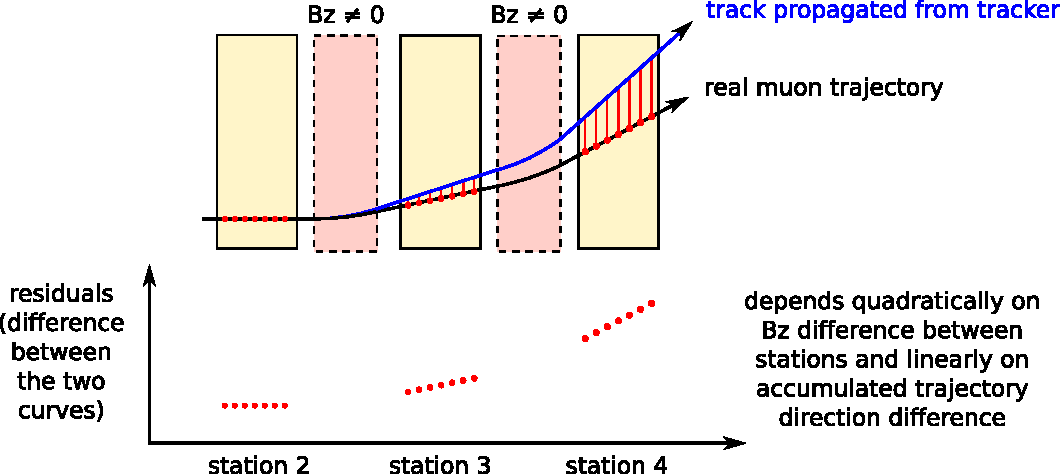
\includegraphics[width=\linewidth]{paths.pdf}

\vfill
\begin{itemize}
\item Gap between propagted track and real muon grows quadratically in yoke when $B_z$ is wrong
\item Gap grows linearly elsewhere, dependent on history

{\scriptsize (This is like a Physics I displacement problem with regions of acceleration)}
\end{itemize}
\end{frame}

\begin{frame}
\frametitle{Effect of $B_z$ errors on segments}

\vfill
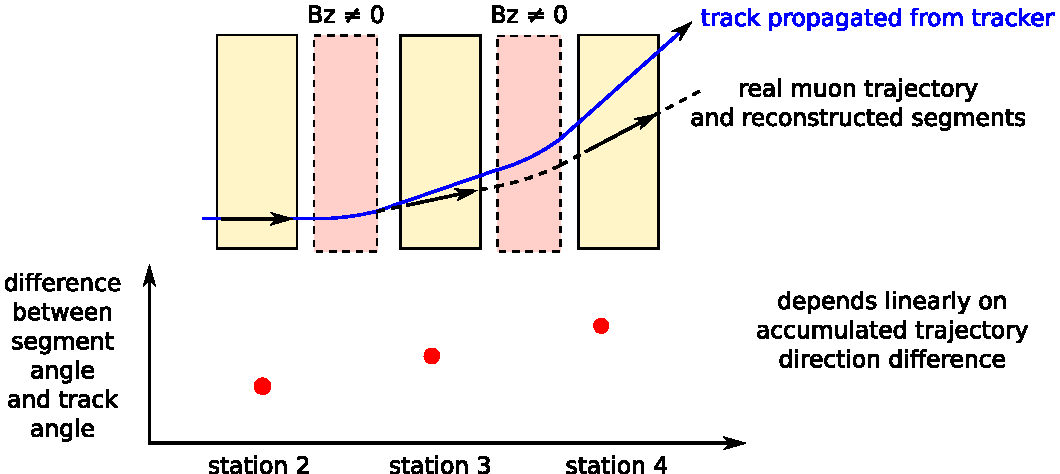
\includegraphics[width=\linewidth]{paths2.pdf}

\vfill
\begin{itemize}
\item Trajectory angle grows linearly in yoke when $B_z$ is wrong

{\scriptsize (This is like a Physics I velocity problem with regions of acceleration)}

\item Difference in segment angles on the same track provides a direct measurement of $B_z$ error
\item Residuals method can provide a cross-check
\end{itemize}
\end{frame}

\begin{frame}
\frametitle{Before correction}

\begin{itemize}
\item Station 4 has the largest $\vec{B}$-field errors: plot residuals across barrel
\item The \textcolor{darkred}{misalignment} breaks cleanly at the \mbox{chamber boundaries\hspace{-1 cm}}
\item The \textcolor{lightblue}{$\vec{B}$-field error} is independent of chamber
\end{itemize}

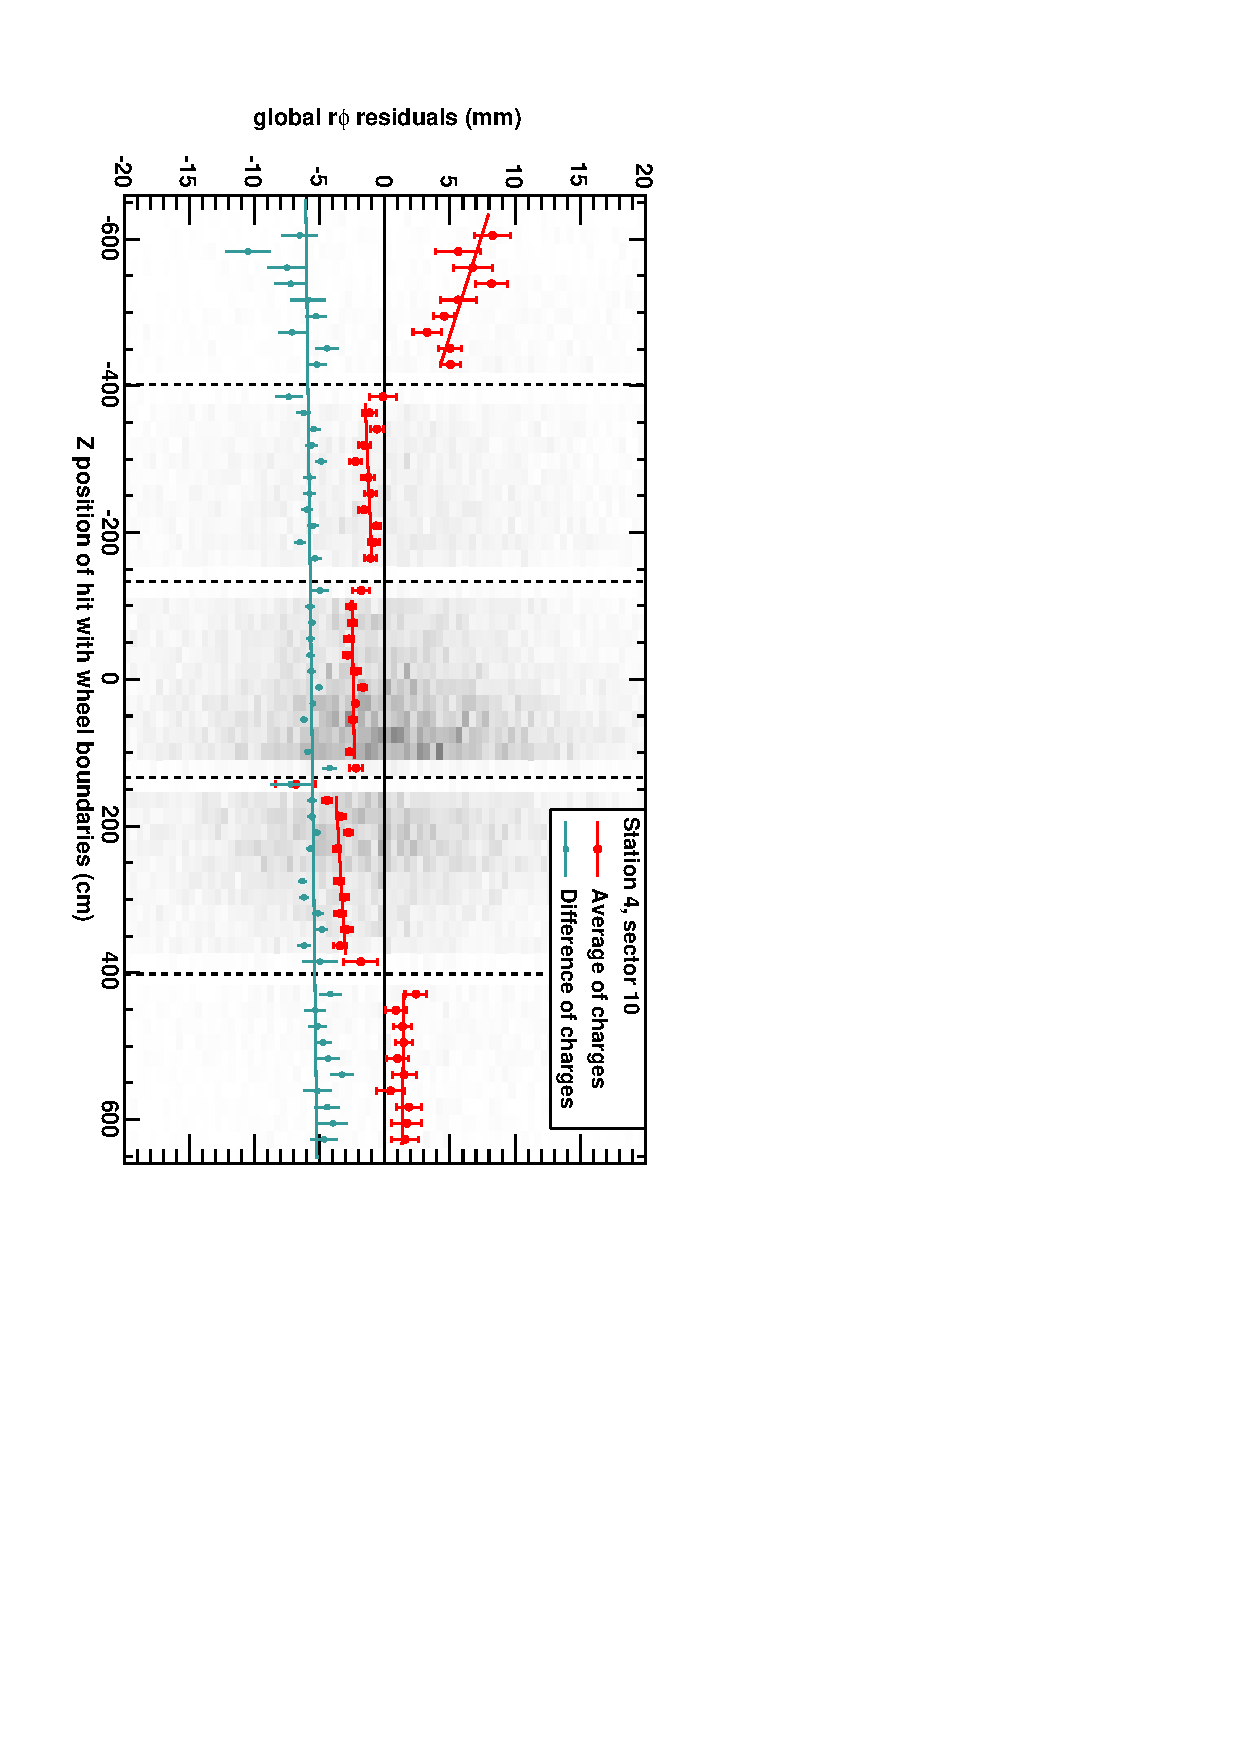
\includegraphics[height=\linewidth, angle=90]{demo_of_bfield.pdf}

\scriptsize grey background is the raw 2-D residuals distribution

linear fits are only a guide for the eye: not used in alignment!
\end{frame}

\begin{frame}
\frametitle{Residuals with new $\vec{B}(\vec{x})$ maps}
\begin{itemize}
\item Two new field maps available:
\begin{itemize}
\item scaling corrections from segments (data-based measurement)
\item new TOSCA simulation (consistent field lines)
\end{itemize}
\item Opportunity to test \textcolor{blue}{correctness of new $\vec{B}(\vec{x})$} and \textcolor{red}{insensitivity of alignment measure} with tracks propagated through new field
\begin{itemize}
\item left: histogram of bins from the previous plot (for all sectors)
\item right: how each bin changes when new field is applied
\end{itemize}
\end{itemize}

\vspace{-0.3 cm}
\mbox{ } \hfill {\tiny statistical errors in bins are ${\mathcal O}(\mbox{0.5~mm})$}

\only<1>{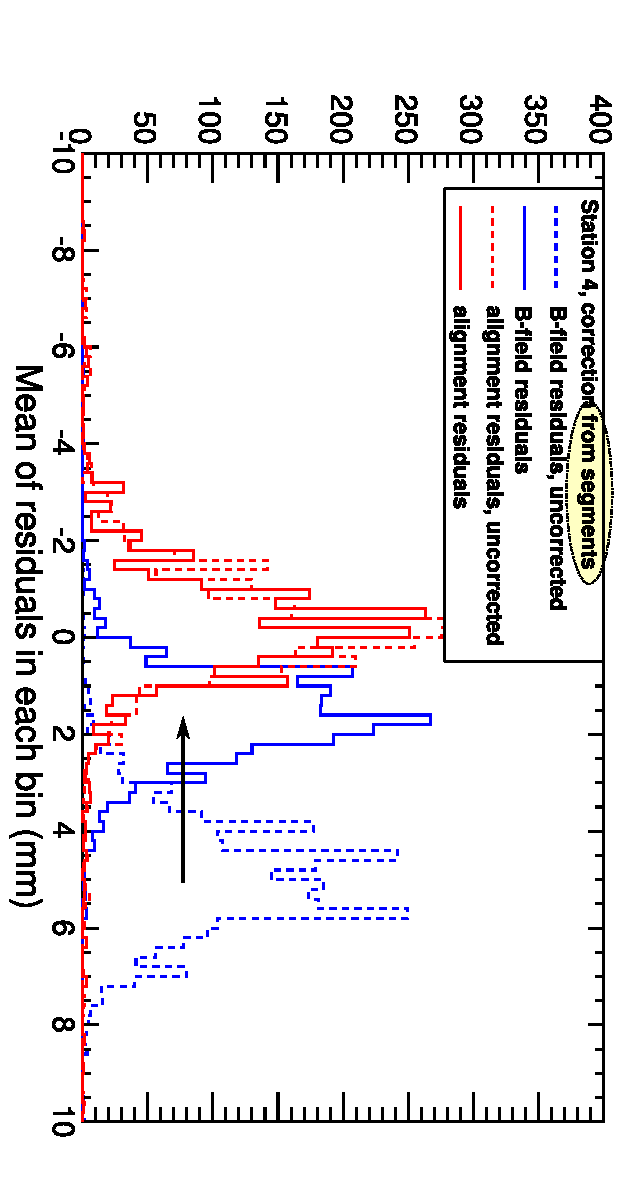
\includegraphics[width=4 cm, angle=90]{scaling_corrections_station4.pdf} 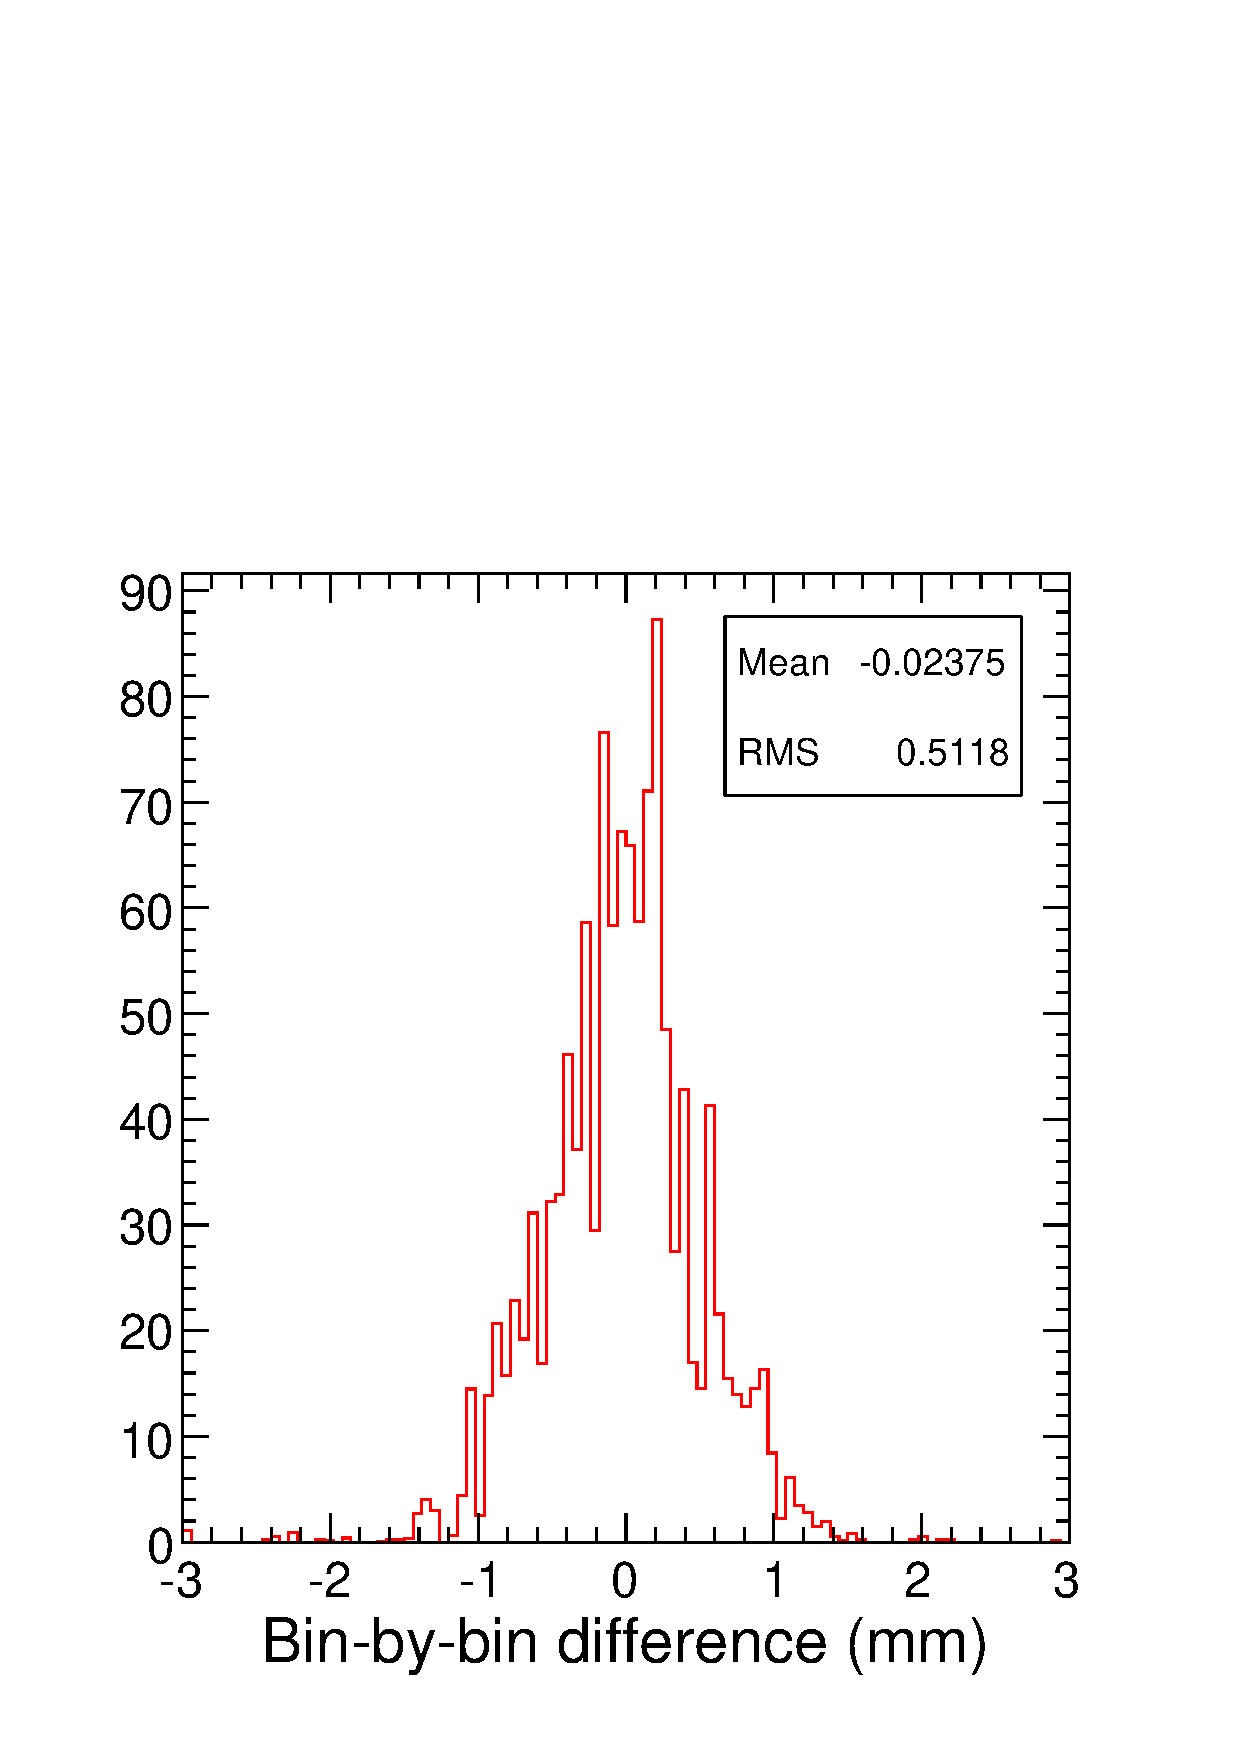
\includegraphics[height=4 cm]{scaling_binbybin_station4.pdf}}
\only<2>{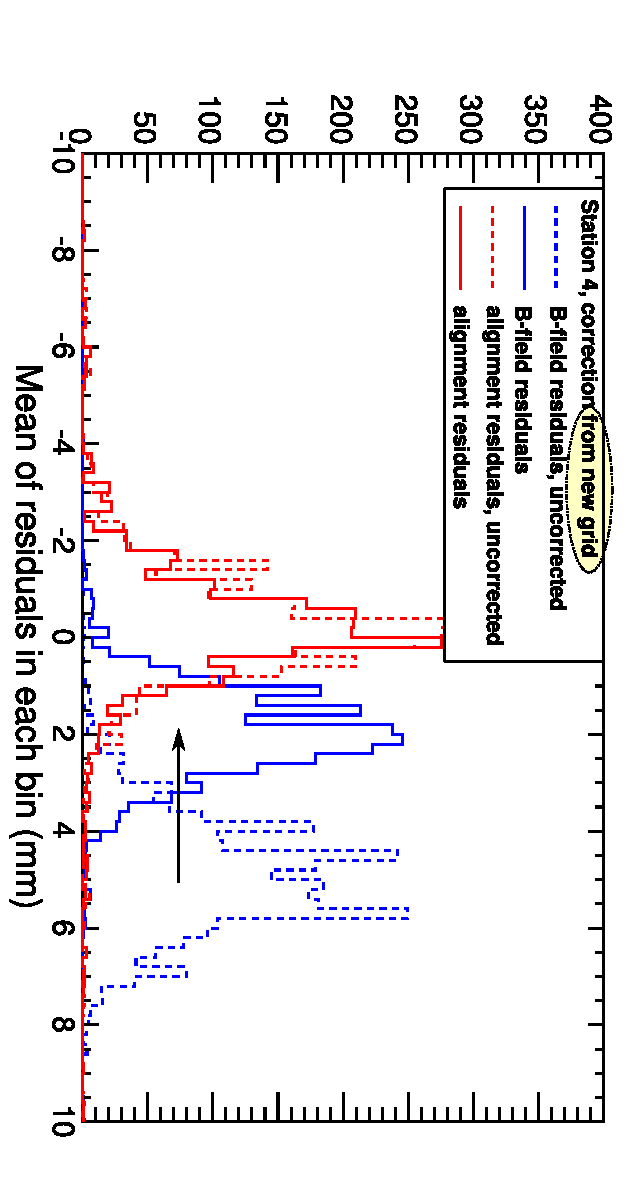
\includegraphics[width=4 cm, angle=90]{newgrid_corrections_station4.pdf} 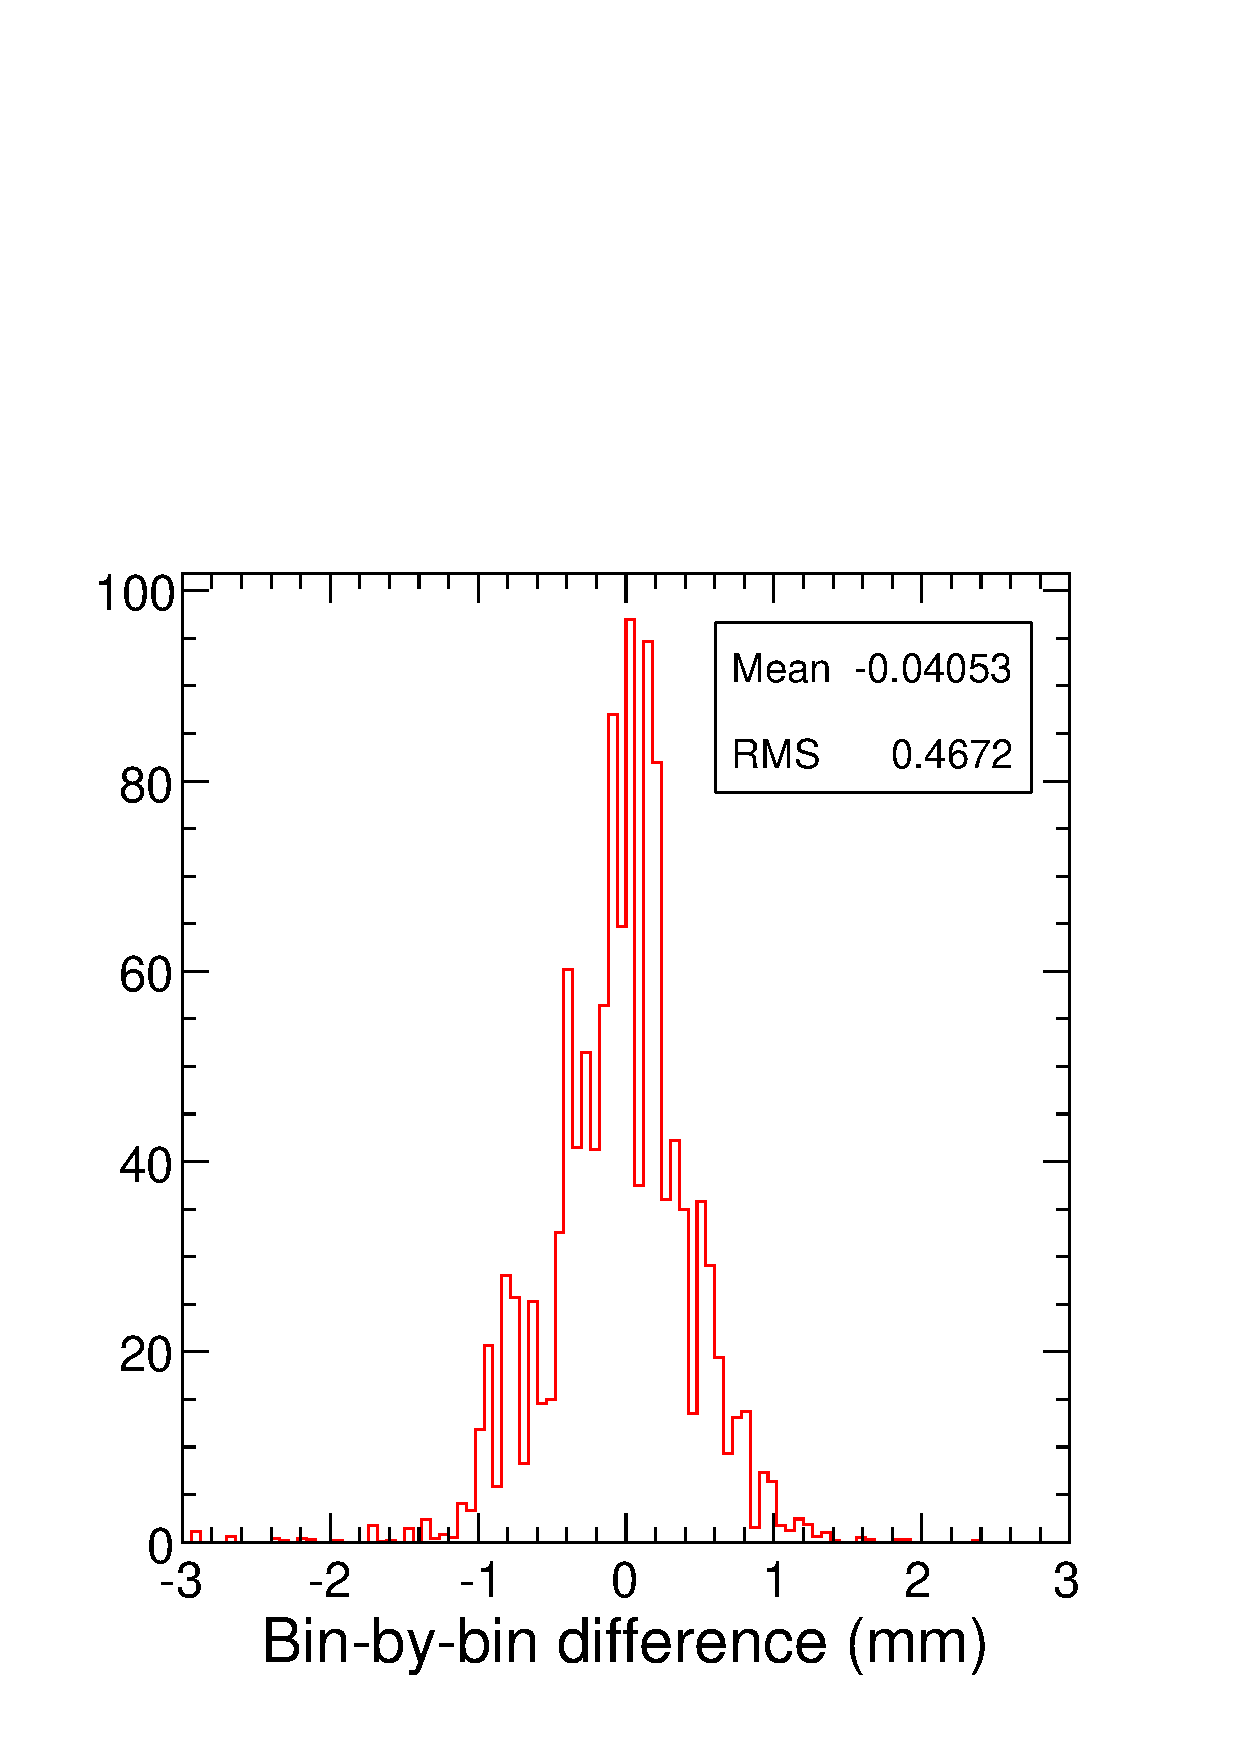
\includegraphics[height=4 cm]{newgrid_binbybin_station4.pdf}}
\end{frame}

\begin{frame}
\frametitle{All four stations: scaling}

\begin{columns}
\column{0.5\linewidth}
Station 1

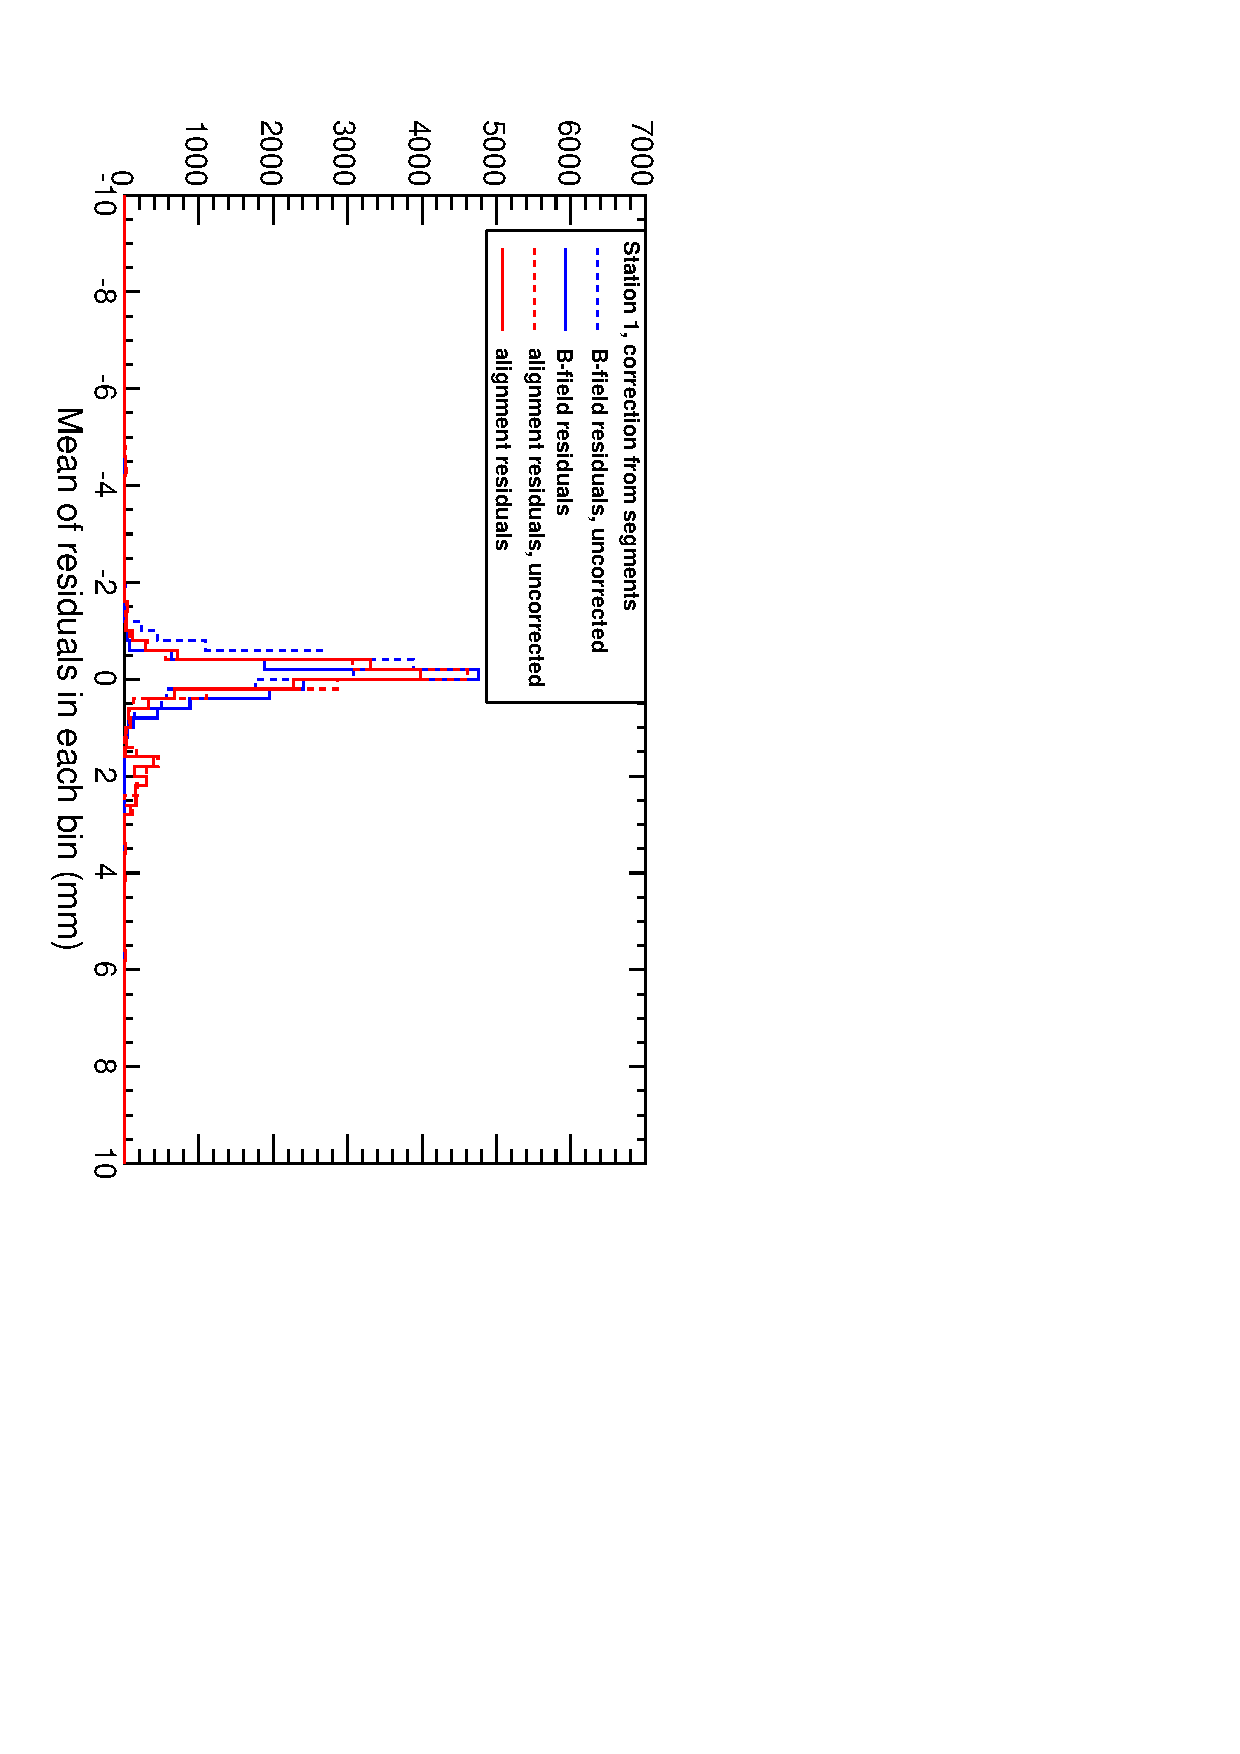
\includegraphics[height=\linewidth, angle=90]{scaling_corrections_station1.pdf}

\vspace{1 cm}
Station 3

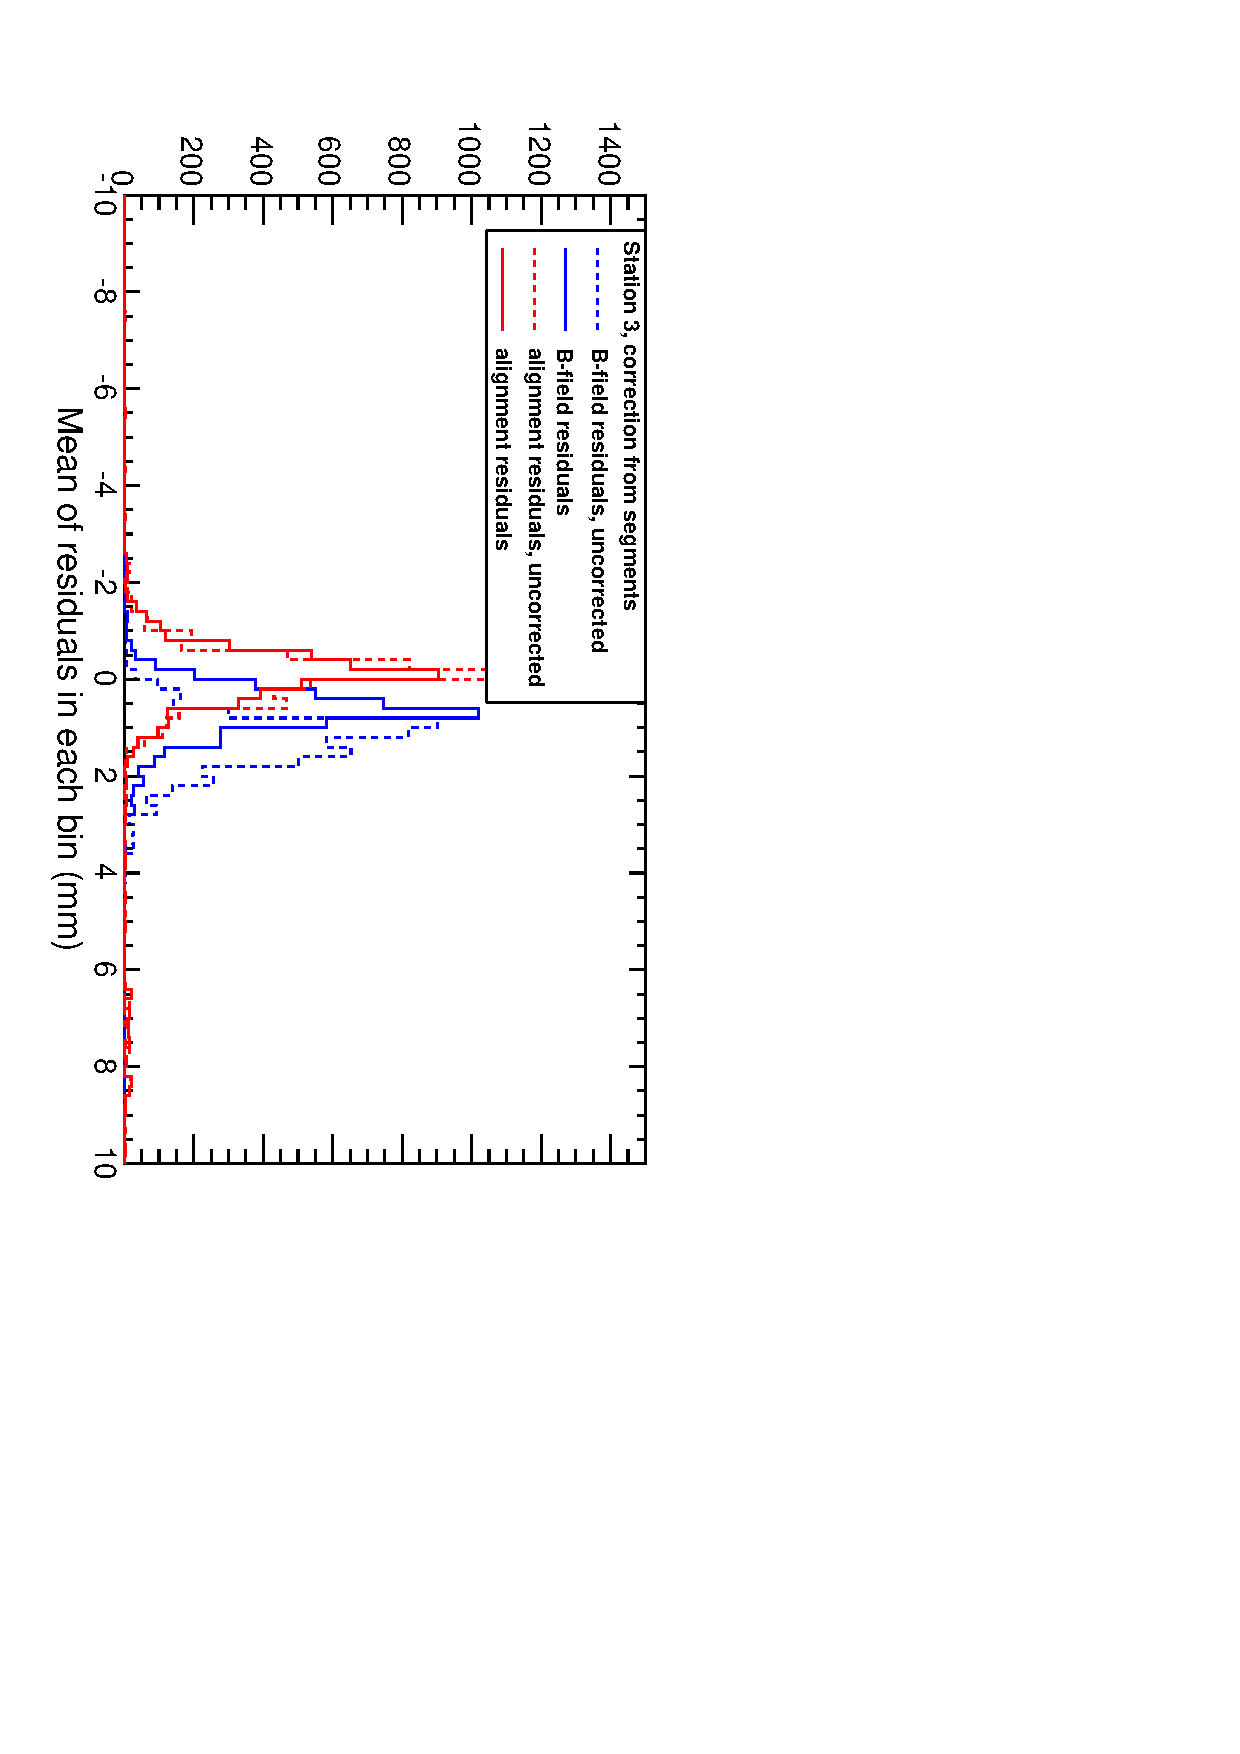
\includegraphics[height=\linewidth, angle=90]{scaling_corrections_station3.pdf}

\column{0.5\linewidth}
Station 2

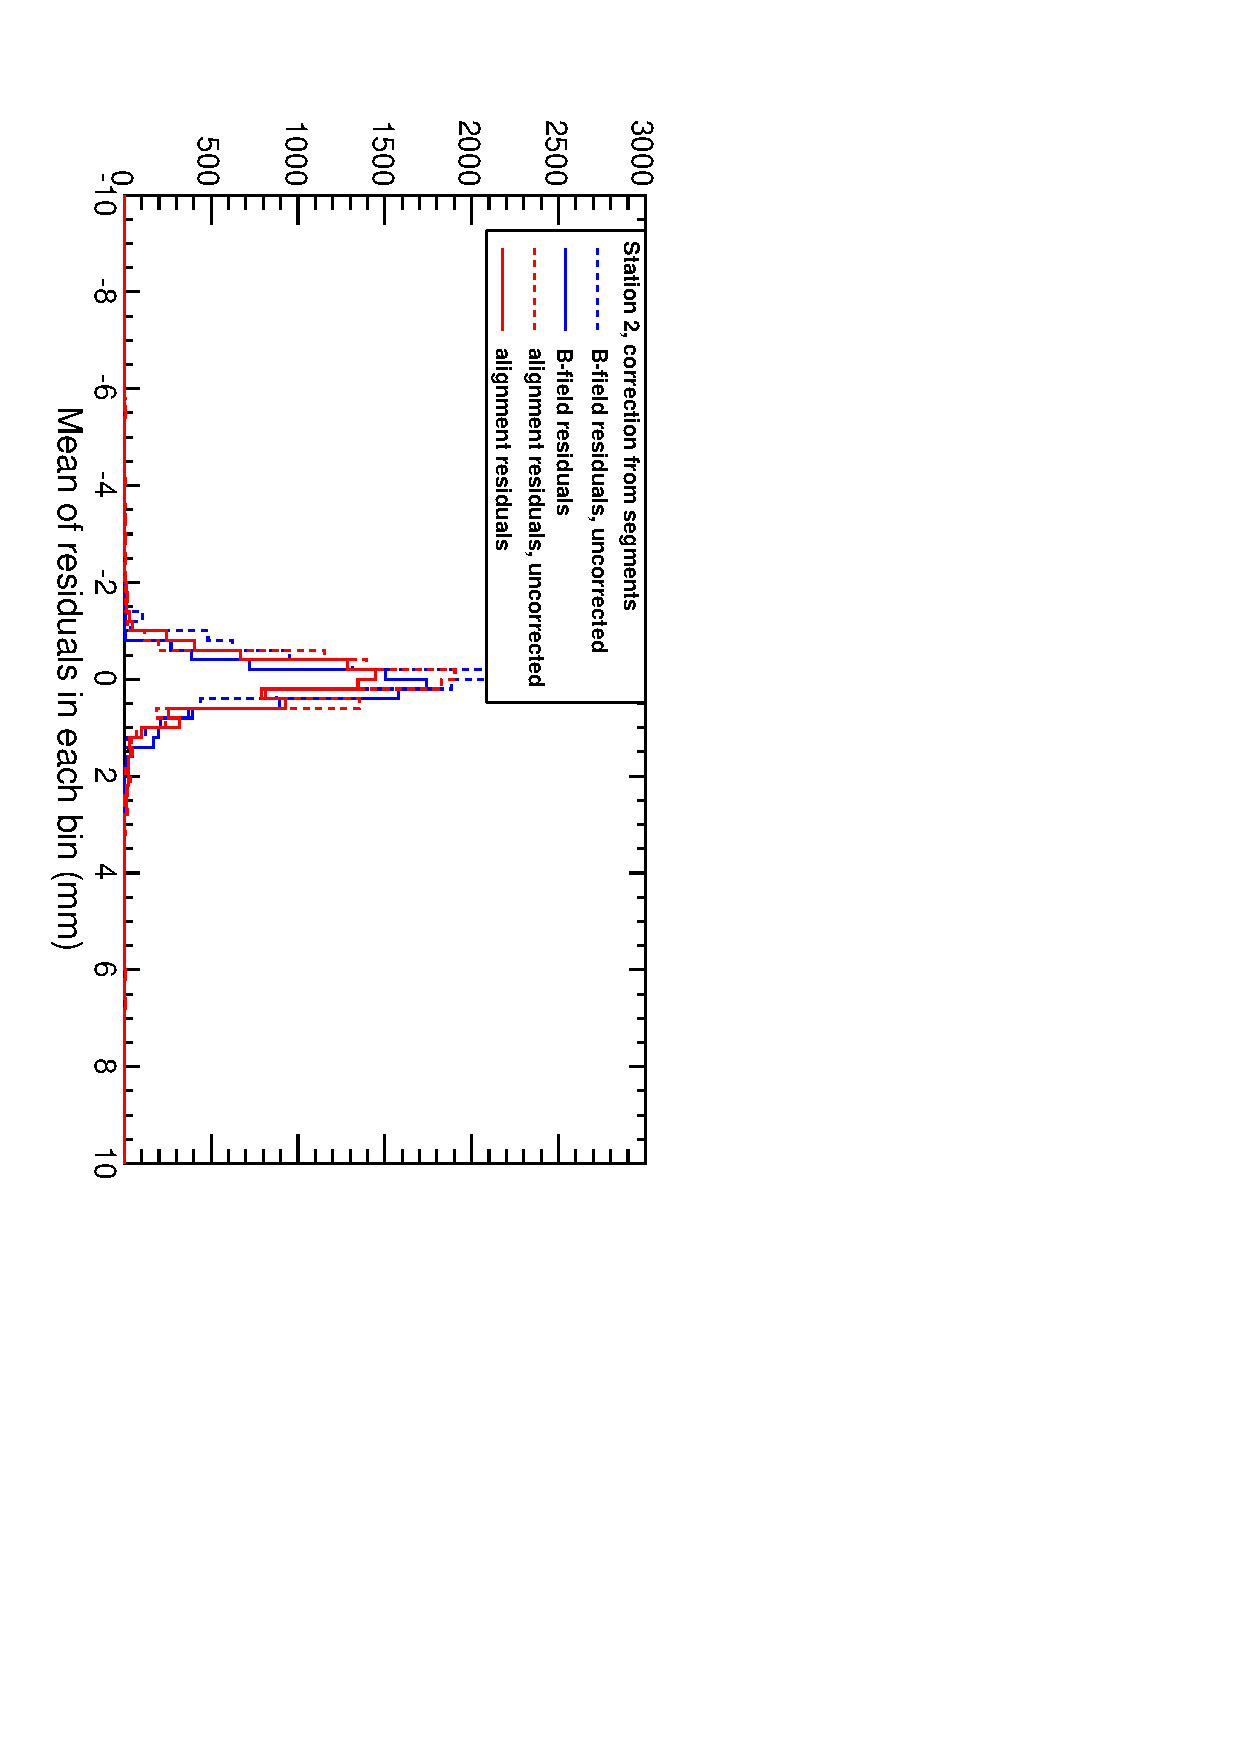
\includegraphics[height=\linewidth, angle=90]{scaling_corrections_station2.pdf}

\vspace{1 cm}
Station 4

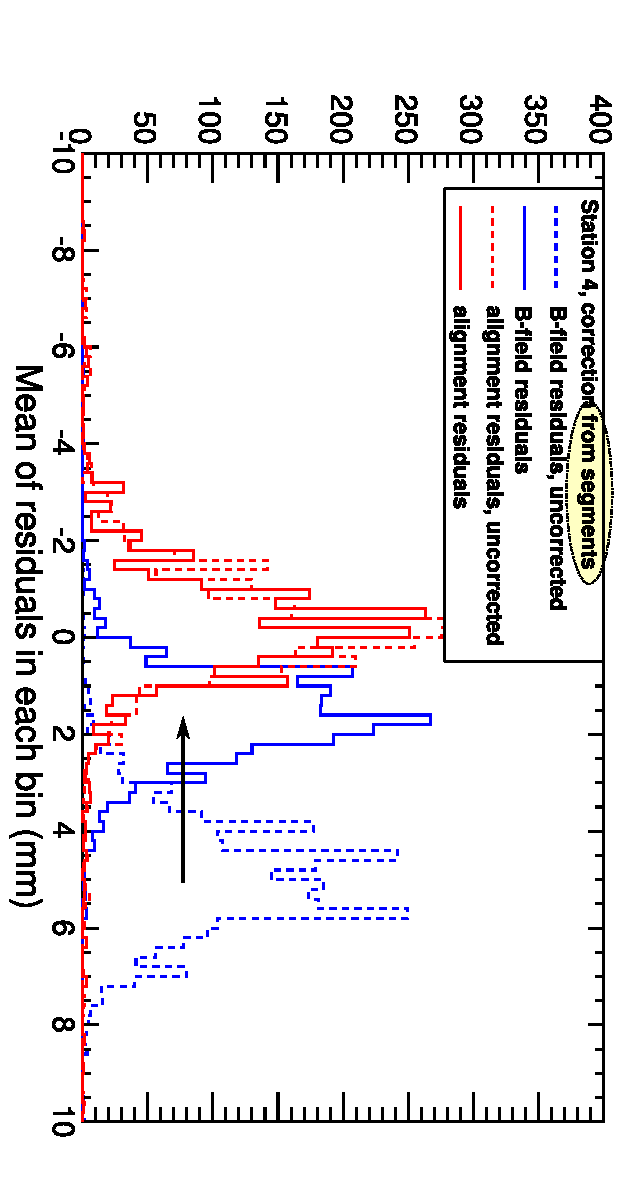
\includegraphics[height=\linewidth, angle=90]{scaling_corrections_station4.pdf}
\end{columns}
\end{frame}

\begin{frame}
\frametitle{All four stations: new grid}

\begin{columns}
\column{0.5\linewidth}
Station 1

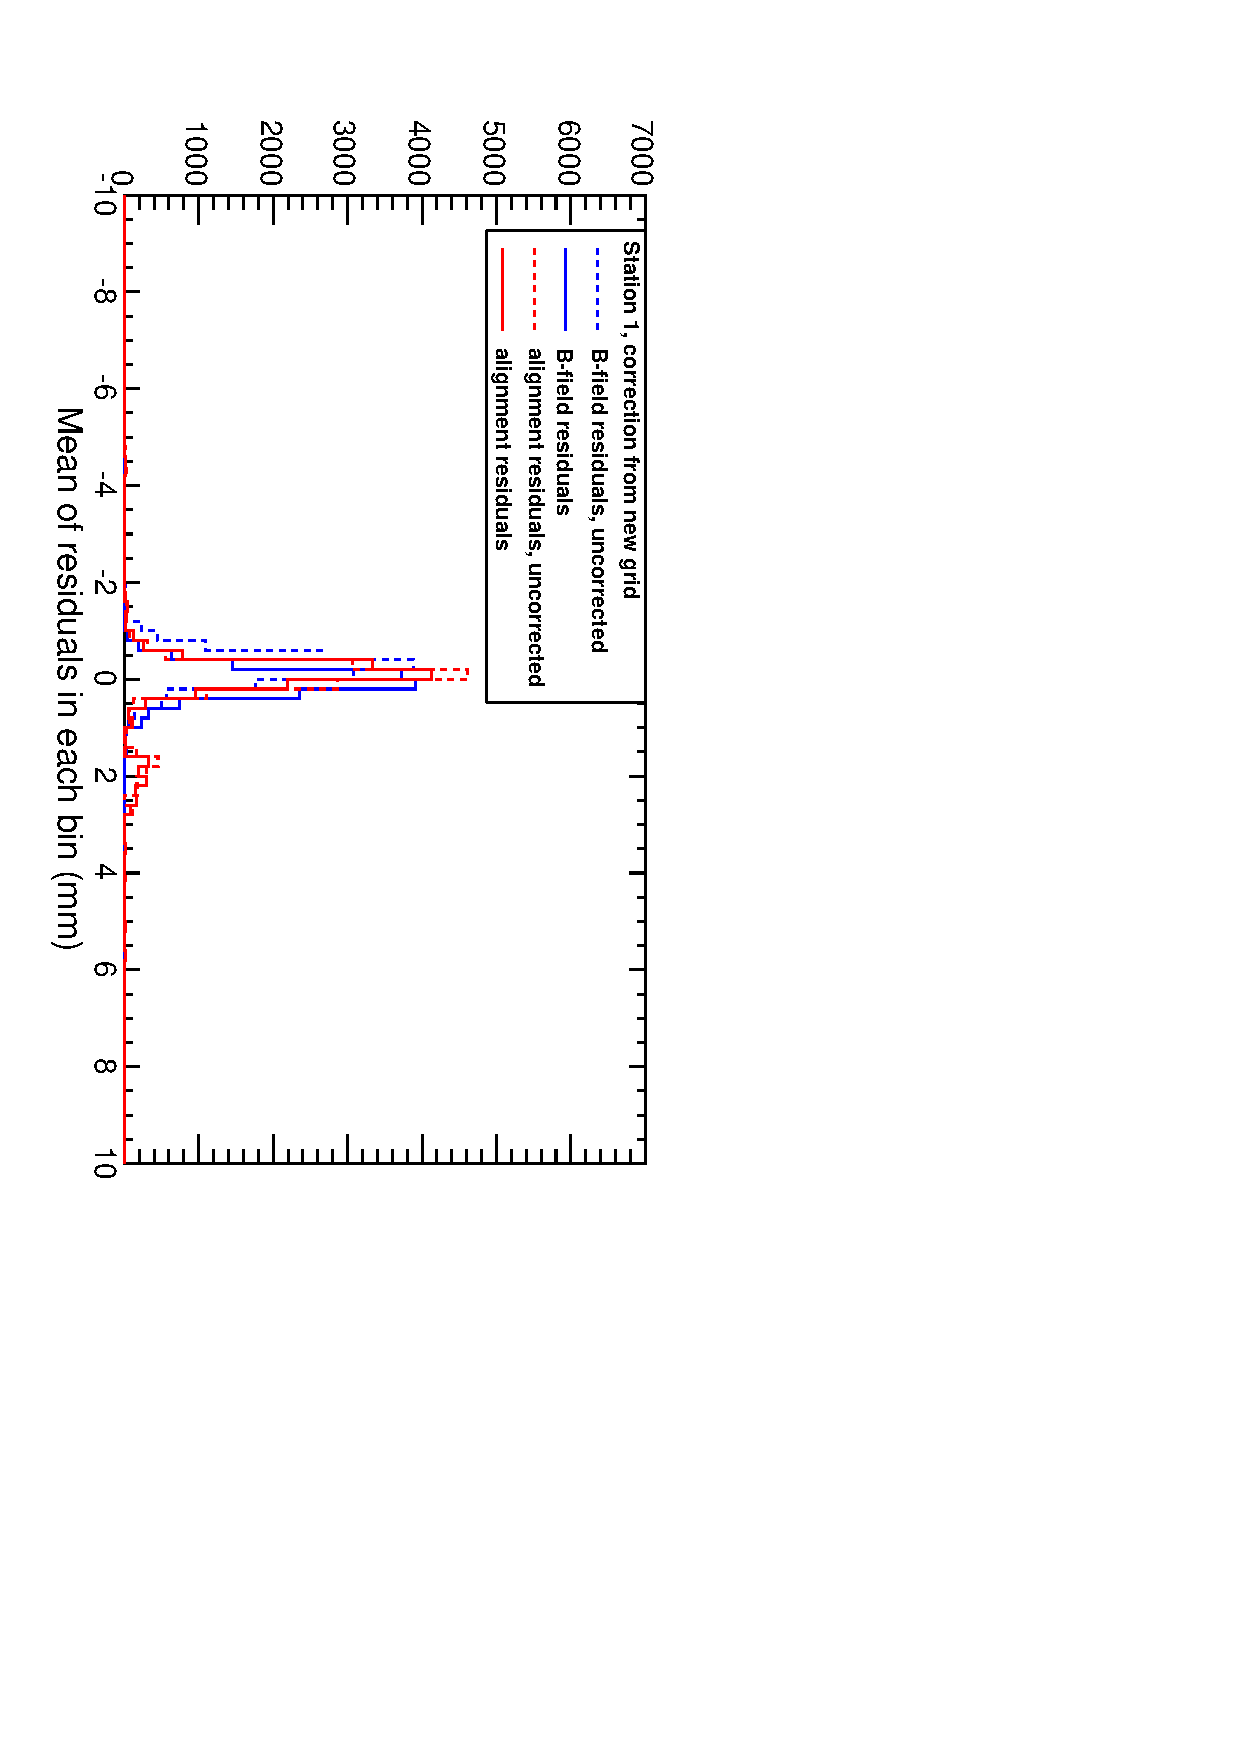
\includegraphics[height=\linewidth, angle=90]{new_grid_station1.pdf}

\vspace{1 cm}
Station 3

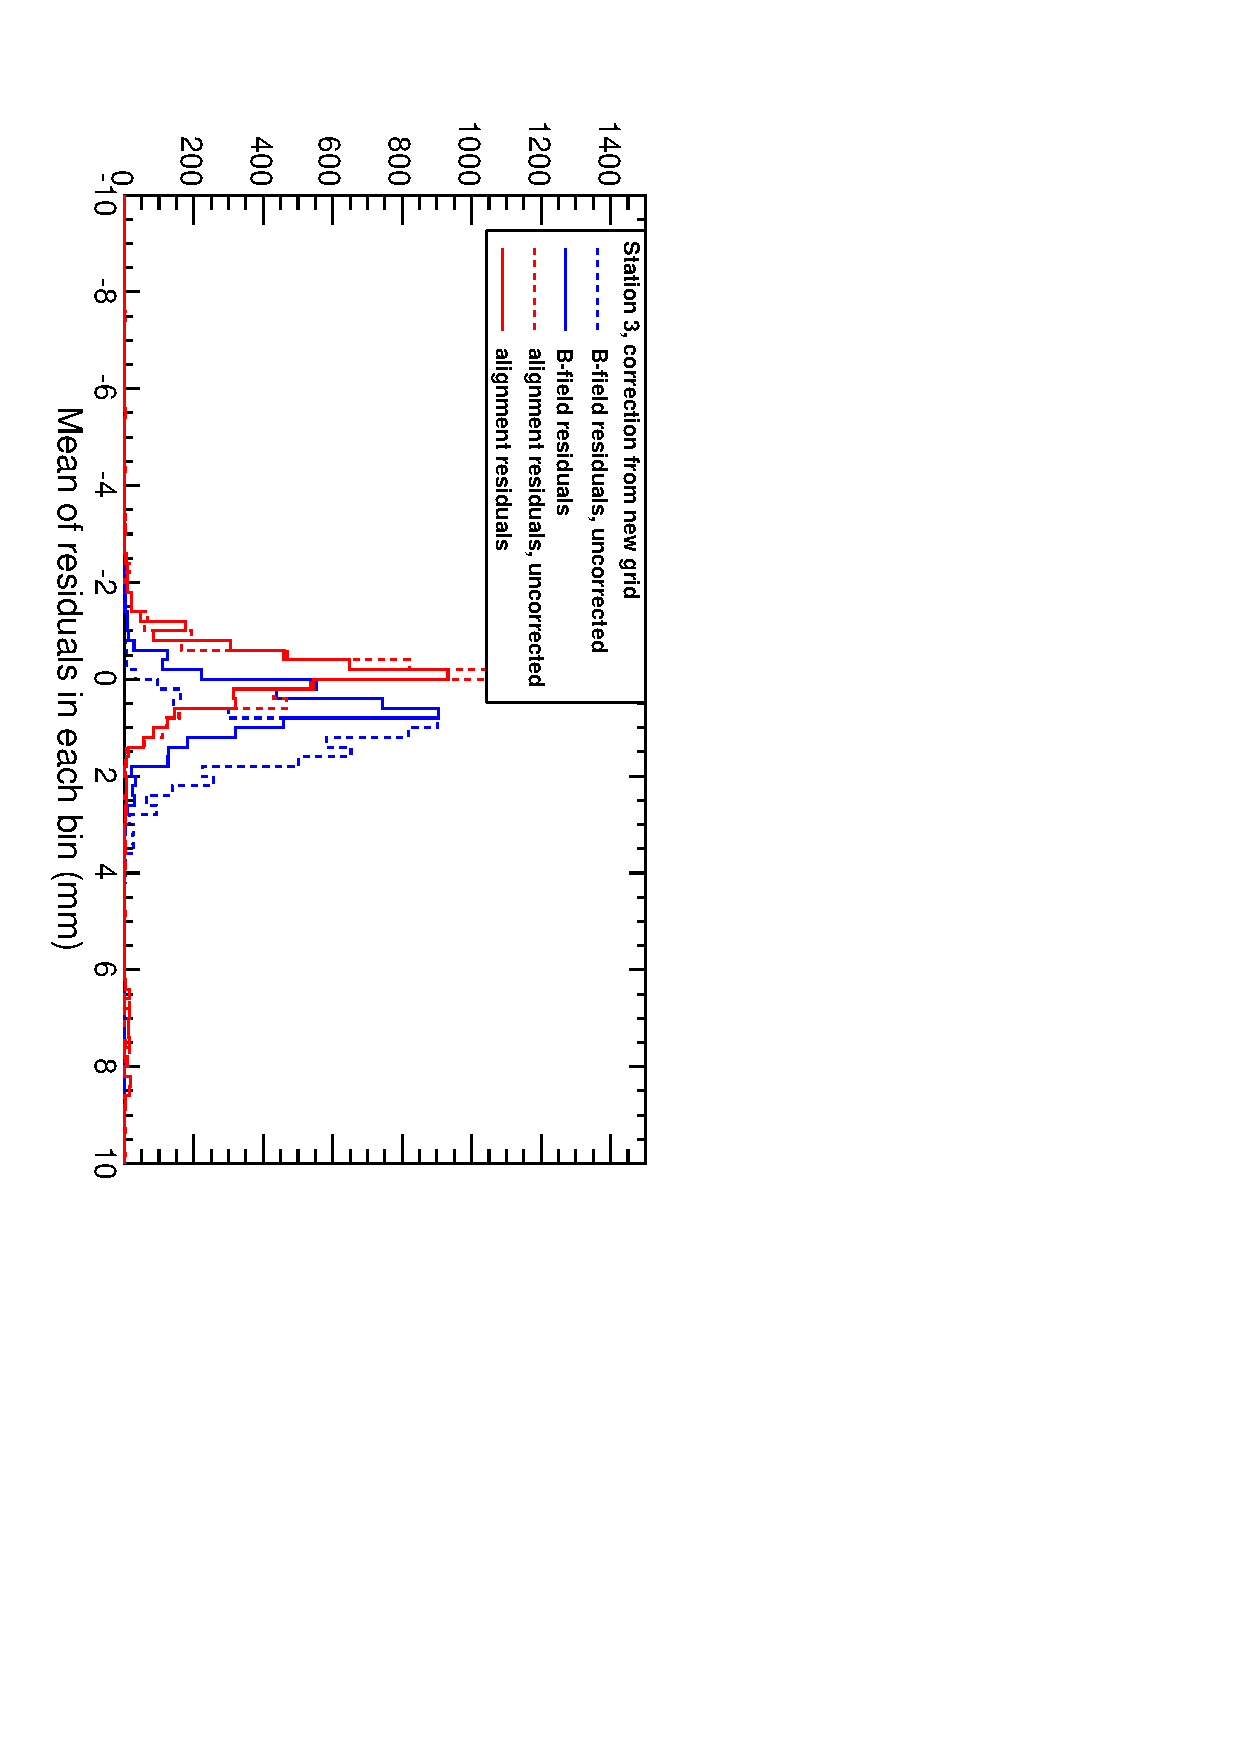
\includegraphics[height=\linewidth, angle=90]{new_grid_station3.pdf}

\column{0.5\linewidth}
Station 2

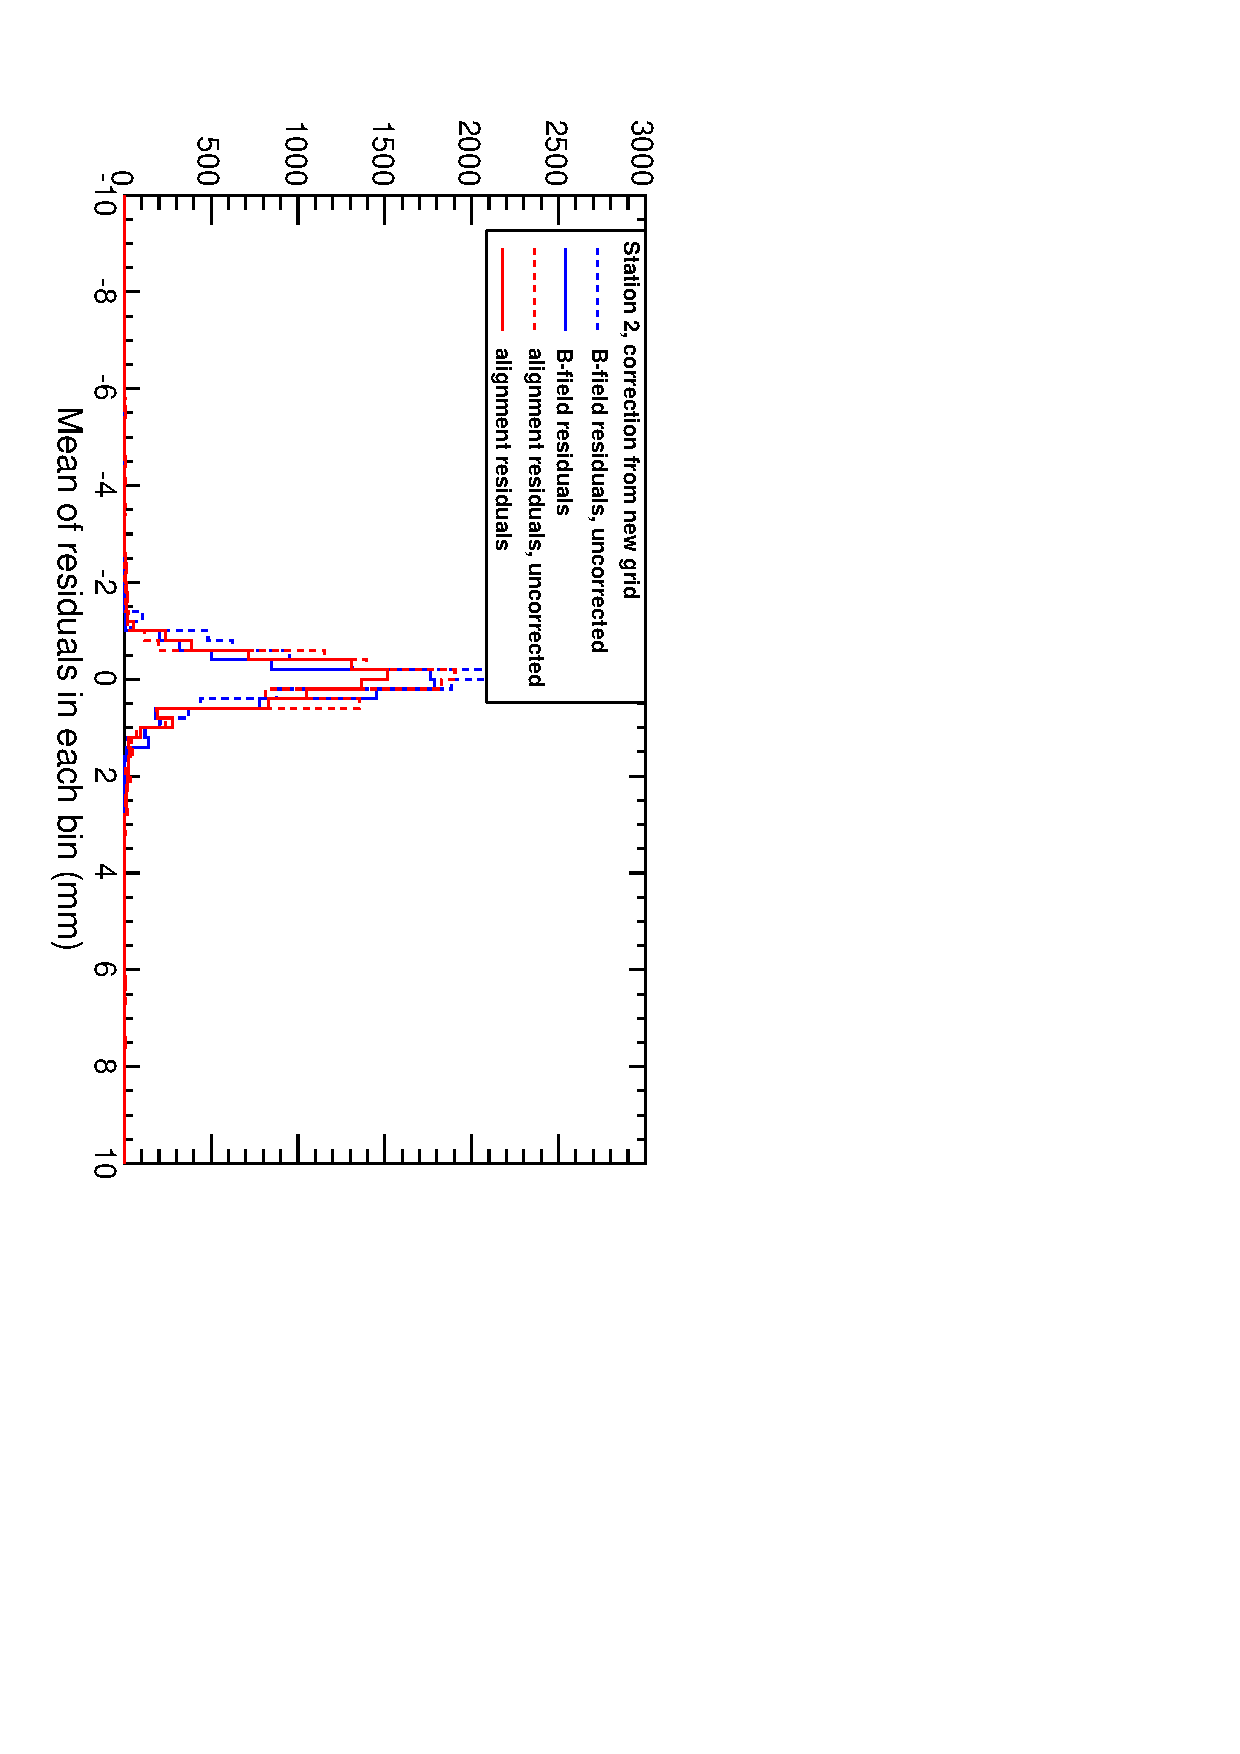
\includegraphics[height=\linewidth, angle=90]{new_grid_station2.pdf}

\vspace{1 cm}
Station 4

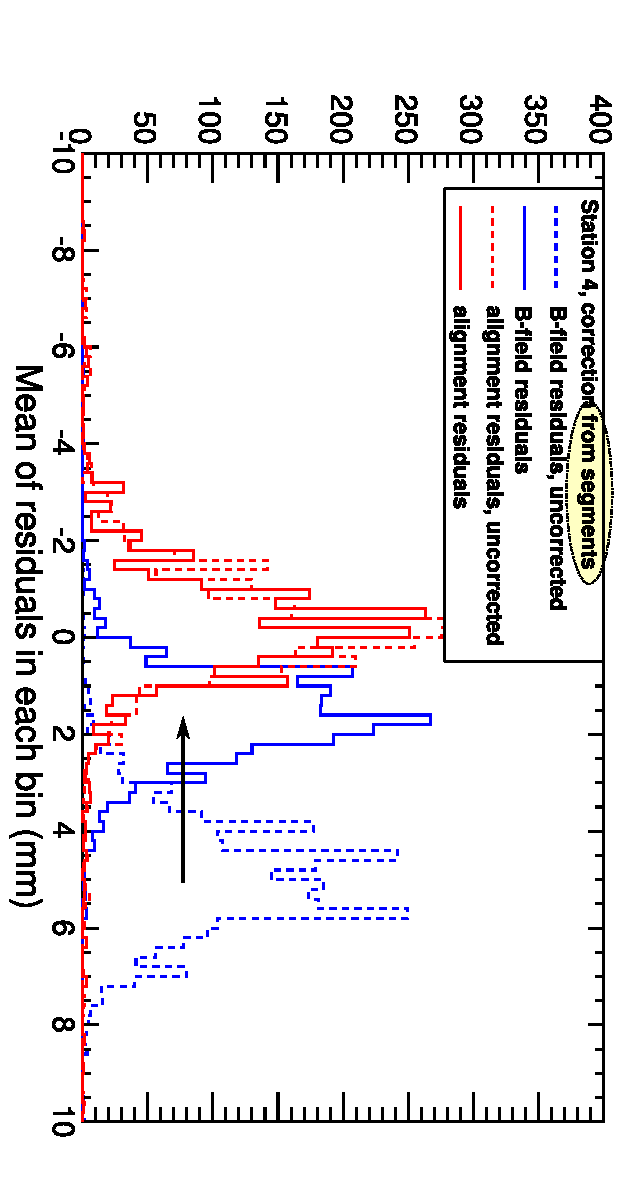
\includegraphics[height=\linewidth, angle=90]{scaling_corrections_station4.pdf}
\end{columns}
\end{frame}

\begin{frame}
\frametitle{Remaining disagreement: $dE/dx$?}

\begin{itemize}
\item $B_z$ error on residuals scales as $q/p_T$
\item $dE/dx$ error on residuals scales as $q\left( \dfrac{1}{p} -
  \dfrac{1}{p - \delta p} \right)$ where $\delta p$ is a constant
  ($\sim$2~GeV/meter of iron if no $dE/dx$ is taken into account,
  exact value will depend on how much is missing
\item Cute feature: $\left(\dfrac{1}{P} - \dfrac{1}{P -
  \delta p}\right) / \left(\dfrac{1}{p} - \dfrac{1}{p - \delta
  p}\right)$ \mbox{$\sim$independent of $\delta p$\hspace{-1 cm}}
\item Cutting cosmic ray spectrum two different $p_T$ values yields
  {\it approximately} similar distributions (differing only by
  scalar multiple)
\end{itemize}

\textcolor{darkblue}{Station 4 from \only<1>{scaling}\only<2>{the new simulation}}

\renewcommand{\arraystretch}{1.25}
\begin{tabular}{c c c c}
$p_T$ cut & expected from $\vec{B}$ error & expected from $dE/dx$ error & \textcolor{darkblue}{observed} \\\hline
20~GeV & 1 & 1 & 1 (def) \\
40~GeV & 0.5 & 0.24 & \only<1>{\textcolor{darkblue}{0.71}}\only<2>{\textcolor{darkblue}{0.69}} \\
80~GeV & 0.25 & 0.06 & \only<1>{\textcolor{darkblue}{0.46}}\only<2>{\textcolor{darkblue}{0.46}} \\
\end{tabular}
\end{frame}


%% \begin{frame}
%% \frametitle{Outline}
%% \begin{itemize}\setlength{\itemsep}{0.25 cm}
%% \item 
%% \end{itemize}
%% %% \hspace{-0.83 cm} \textcolor{darkblue}{\Large Outline2}
%% \end{frame}

%% \section*{First section}
%% \begin{frame}
%% \begin{center}
%% \Huge \textcolor{blue}{First section}
%% \end{center}
%% \end{frame}

\begin{frame}
\frametitle{Conclusions}
\begin{itemize}
\item Residuals method is rather different from segments method: more
  sensitive and more difficult to interperet
\item Scaling from segments and new TOSCA map yield nearly the same
  improvement in residuals: corrected more than half of the effect
\item Remaining effect is not dominated by $dE/dx$ errors
\end{itemize}

\vfill
\begin{itemize}
\item Special feature!  On the next four pages, I present some tools
  that will likely be useful for future $\vec{B}$ studies
\end{itemize}
\label{numpages}
\end{frame}

\begin{frame}
\frametitle{Motivation}
\begin{itemize}
\item Residuals distributions have power-law tails due to single-scattering
\item Especially angular distributions
\item Peak-fit is more precise than mean
\item $\phi_y$ is the angle with $\vec{B}$-field information \mbox{(perfectly aligned MC below)\hspace{-1 cm}}
\end{itemize}
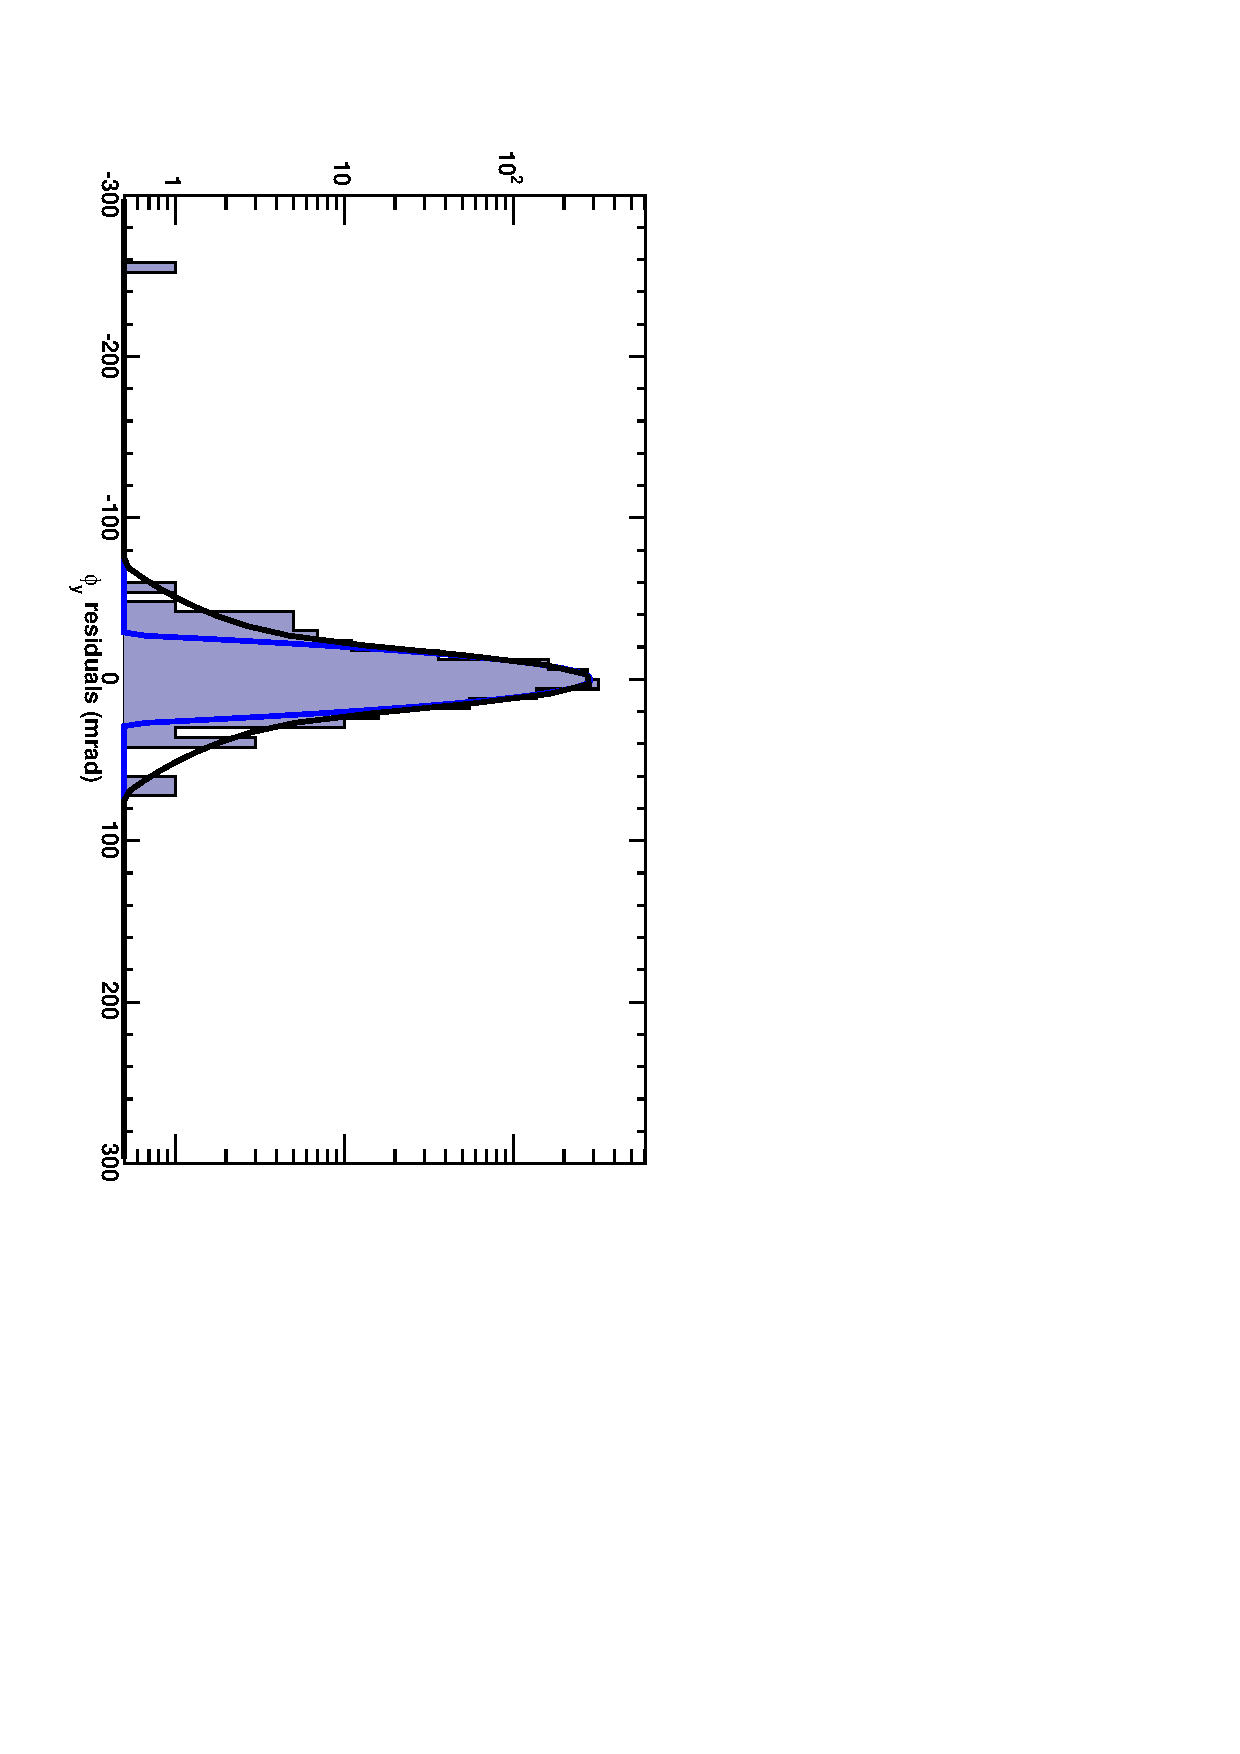
\includegraphics[height=\linewidth, angle=90]{phiy_with_tails.pdf}
\end{frame}

\begin{frame}
\frametitle{More motivation}

\begin{columns}
\column{0.4\linewidth}
\hfill 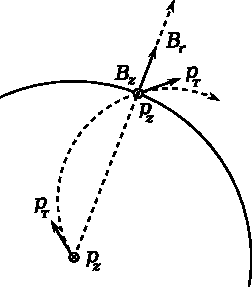
\includegraphics[width=0.6\linewidth]{bfield_components.pdf}

\vspace{0.5 cm}
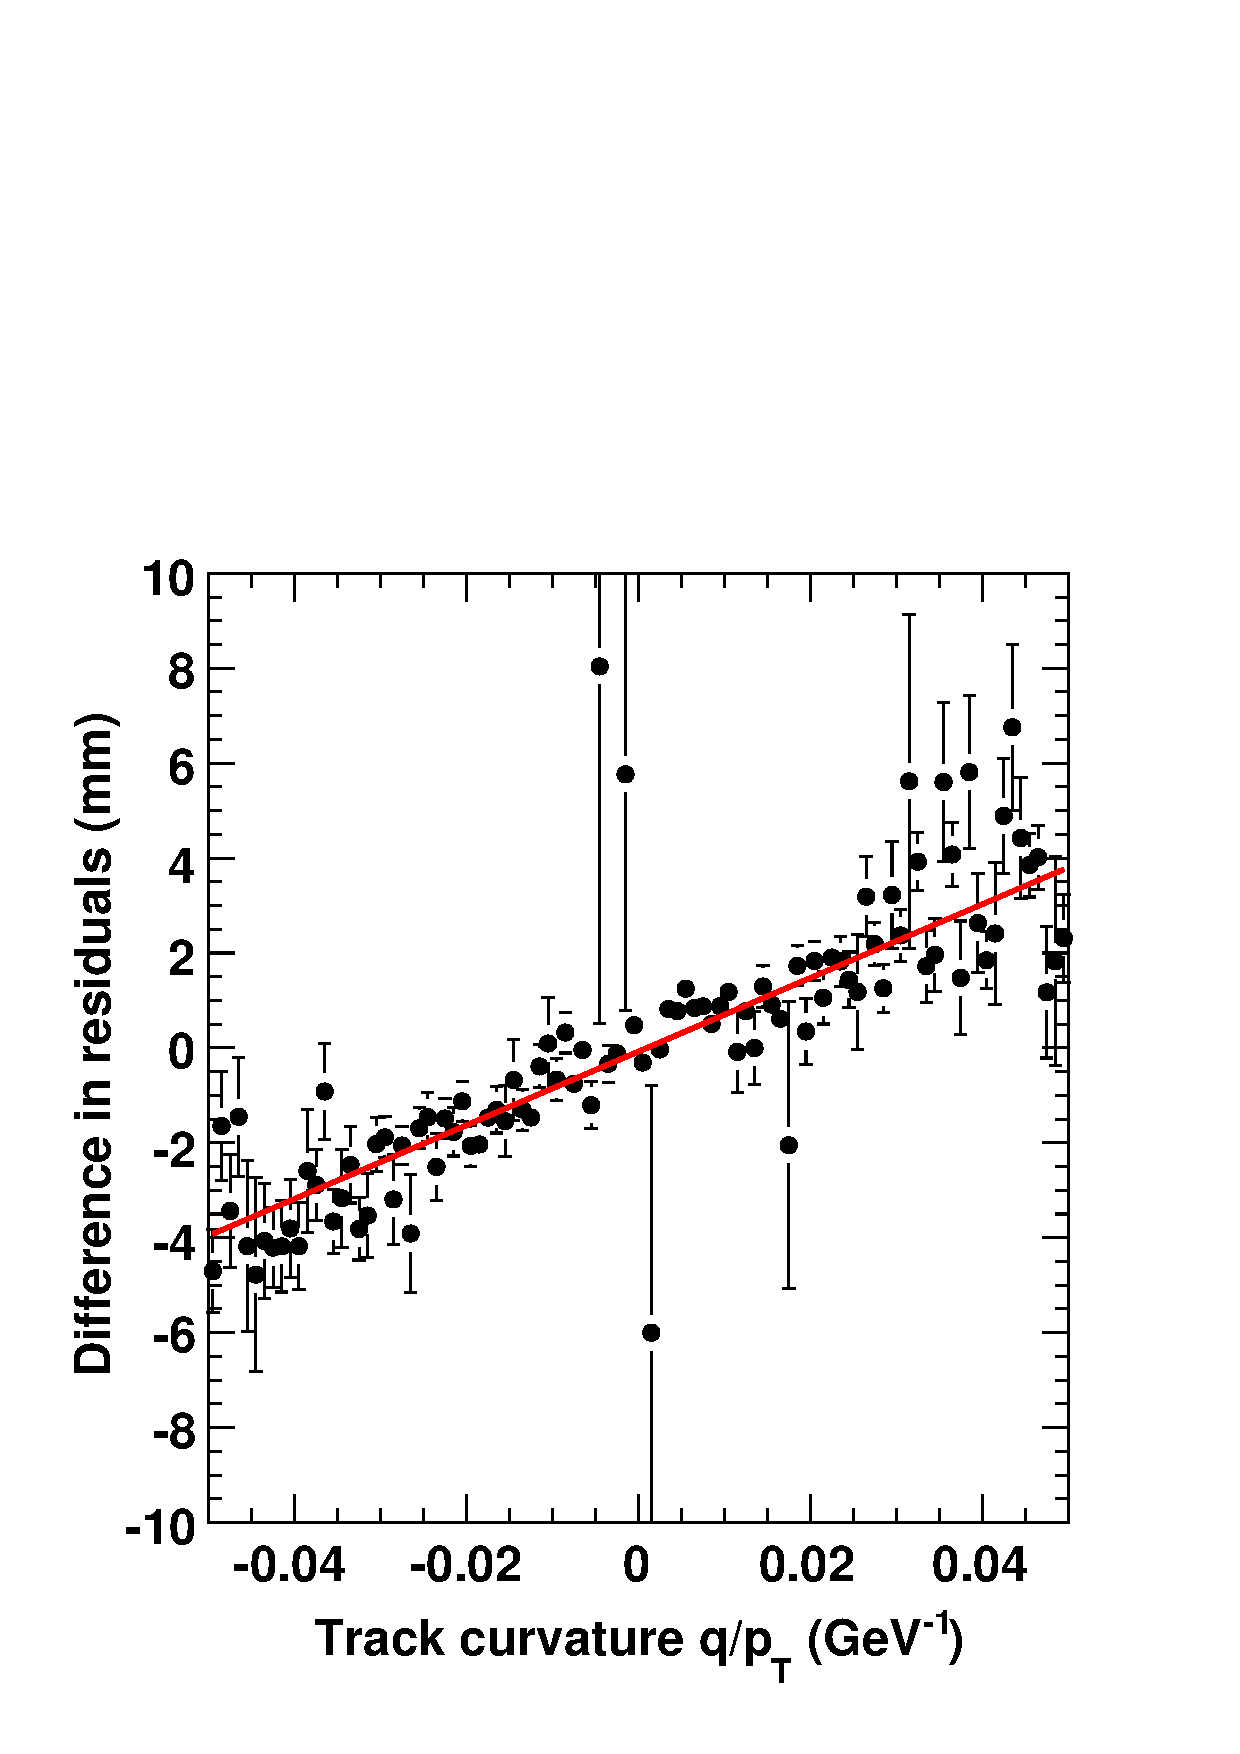
\includegraphics[width=\linewidth]{demo_qoverpt.pdf}
\column{0.6\linewidth}
\begin{itemize}
\item We know that $r\phi$ residuals from a $B_z$ error are linear in $q/p_T$
\item The same residuals are affected by $B_r$ errors, linear in $q/p_z$
\item In a region with both types of $\vec{B}$ error (endcap,
  especially), one would want to disambiguate them with a two-parameter fit
\item Tools in CVS perform fits with Gaussian $\oplus$ tails {\it and}
  linear trends in the crest
\item Example on the left is Gaussian $\oplus$ tails with a $q/p_T$ slope (NOT a linear fit to the profile plot)

source: cosmic ray difference between stations 3 and 4

\end{itemize}
\end{columns}
\end{frame}

\begin{frame}
\frametitle{State of the new tools}
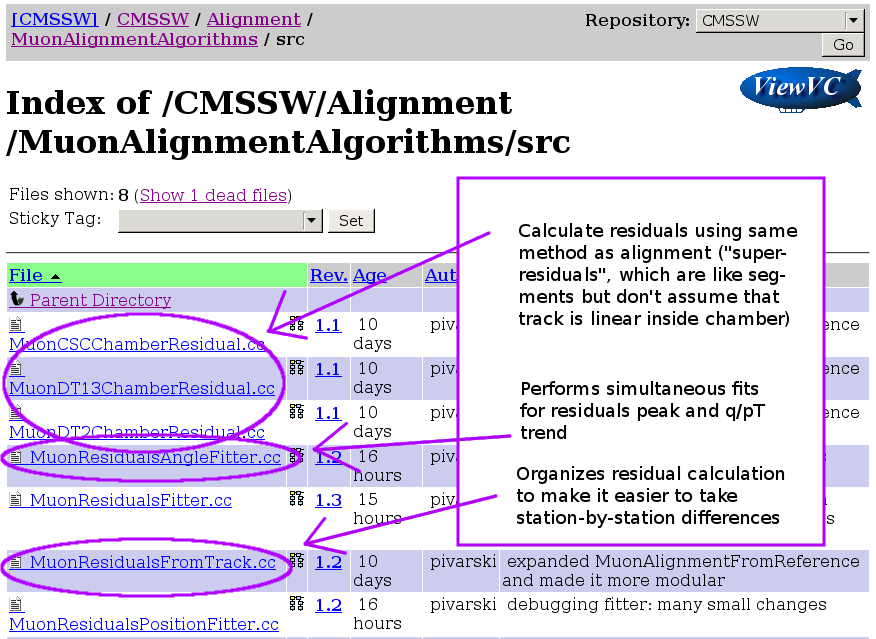
\includegraphics[width=\linewidth]{cvs.png}
\end{frame}

\begin{frame}
\frametitle{Significant $B_r$}
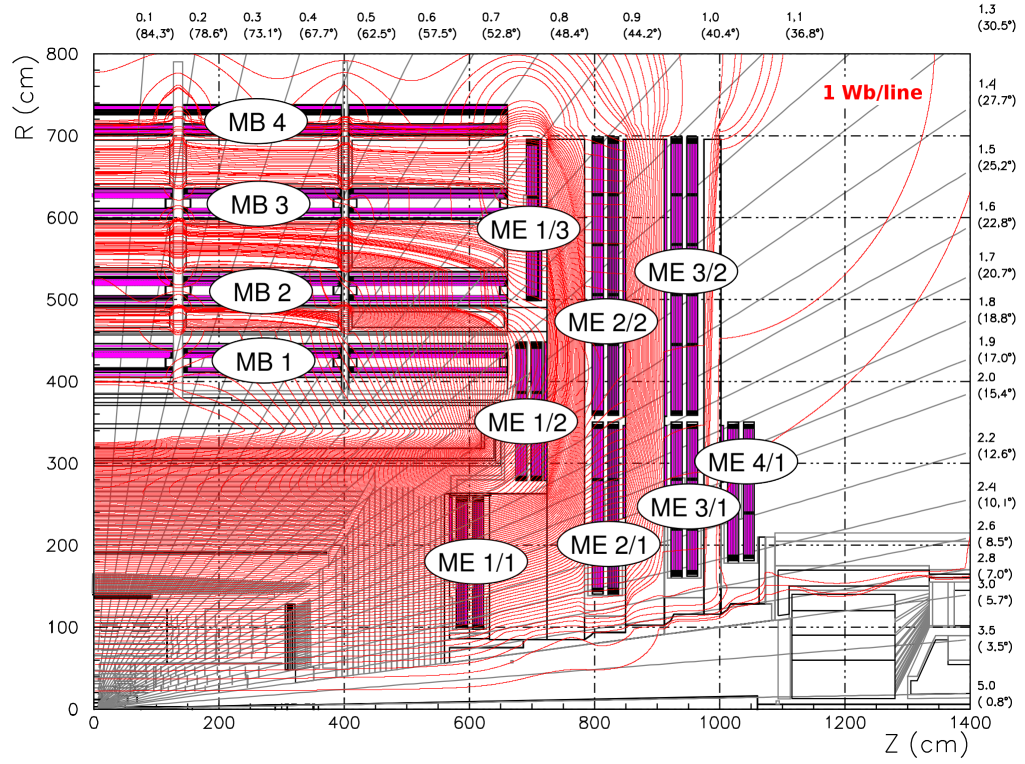
\includegraphics[width=\linewidth]{muon_system_with_lines.png}
\end{frame}

\end{document}
